\documentclass[]{article}
\usepackage{graphicx}
\graphicspath{{/home/john/Documents/Python/Networks} }
%opening
\title{Network Project}
\author{}

\begin{document}

\maketitle

\begin{abstract}

\end{abstract}

\section{Implementation of the BA Model}
\subsection{The Initial Conditions}
The BA model is a randomly generated model, which usees a mdethod called preferential attachement to favour which nodes to connect to. This means that nodes with a high degree are more likely to be attached to be new nodes. The algorithm I used works as follows:
1. Set of an initial network a time $\mathcal{G_0}$.\\
\newline
2.Increment time t $\rightarrow$ t+1\\
\newline
3.Add one new vertex.
4. Add m edges as follows..
....\\...\\..\\
There are a few points of ambiguity in this model. The first of which is with respect to $\mathcal{G}_0$. There is no explicit guidance on how to choose $\mathcal{G}_0\!$, however the choice of starting graph does have an affect. When deriving a solving the master equation for the system, we will use the approximation that $E(t)=mN(t) \!for\! large\! t$. However we can make this approximation exact by choosing an $\mathcal{G}_0$ such that $E(0)=mN(0)$.\\
In finding this, one assumption I would like to make is that ever node in $\mathcal{G_0}$ has the same degree. This make an easily programmably starting graph.This implies that $deg(n)=m\! for\! n \in \mathcal{G_0}$\\
There are many graphs with this property, however I would like to minimise the number of nodes in my starting graph(So our starting graph does not change our statistic) which implies we want a complete graph. THe algebra is as follow:
In a complete graph $E=\sum_{n=1}^{N} n-1 = \frac{N(N-1)}{2}$\\
\vspace{0.2cm}
And so $E(0)=mN(0) \Rightarrow \frac{N(0)(N(0)-1)}{2}=mN(0)$\\
\vspace{0.2cm}
$\Rightarrow N(0)^2 - (2m -1)N = 0$\\
\vspace{0.2cm}
$\Rightarrow N=0 (trivial) and N=2m+1$\\
\vspace{0.2cm}
Therefore choosing $\mathcal{G}_0$ to be a complete graph with $2m+1$ nodes is sufficient for the condition $E(0)=mN(0)$. Figure 1.1 shows the initial networks. 
\begin{figure}[htp]
	\centering
	%\includegraphics{figure_1.png}
	
	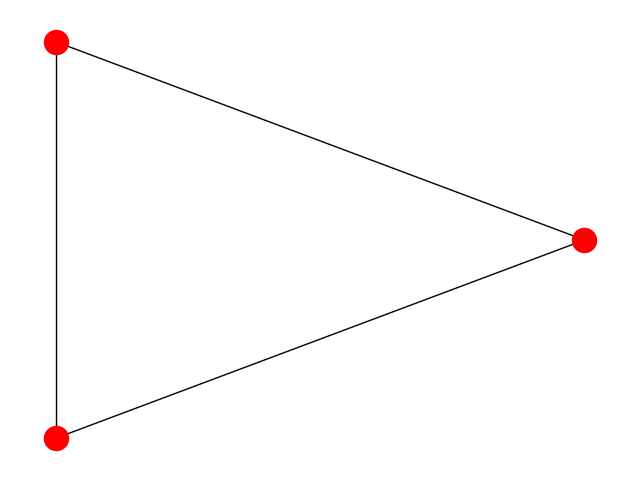
\includegraphics[width=.3\textwidth]{G0m=1.png}\hfill
	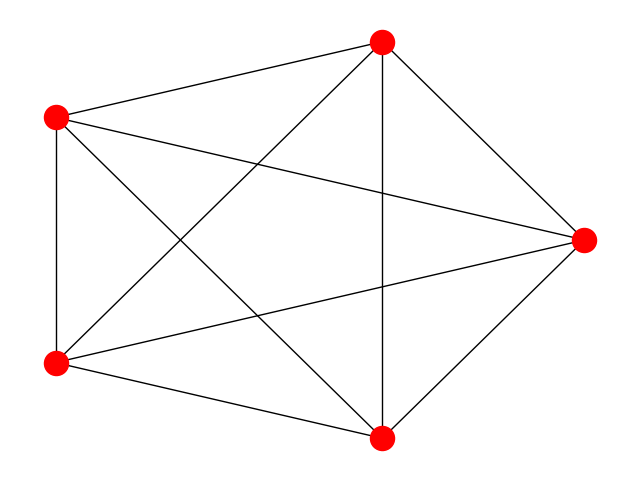
\includegraphics[width=.3\textwidth]{G0m=2.png}\hfill
	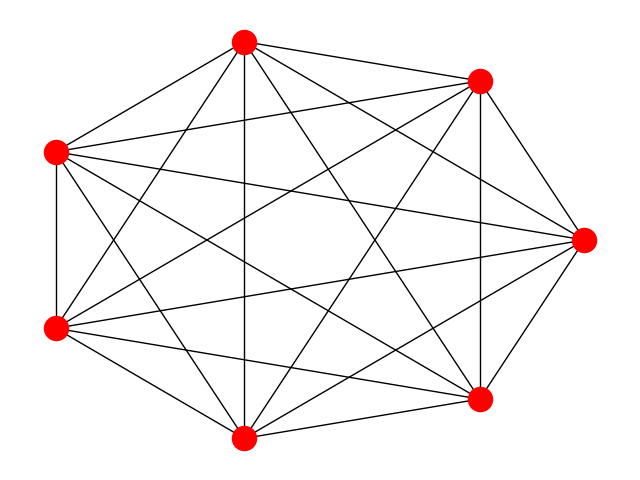
\includegraphics[width=.3\textwidth]{G0m=3.png}
	\caption{\textit{$\mathcal{G}_0$ for m=1,2,3 respectively.}}
\end{figure}
\subsection{Double Edges}
Another point of ambiguity is with regards to multiple egdes. In  the model, we have preferential attachement, which implies as we attach more edges to a node, it will be preferred even more when adding the node edge randomly. This "Rich get richer" attitude means that we are likely to get double edges when $m>1$. For instance, if a new node $k$ is added and attached to node $n<k$, then the probability of that happening again rises, implying we are more likely to see a double edge. This is especially true for small networks. Figure 1 shows a graph of 10 without addressing this issue and one where we do.
\begin{figure}[htp]
	\centering
	%\includegraphics{figure_1.png}
	
	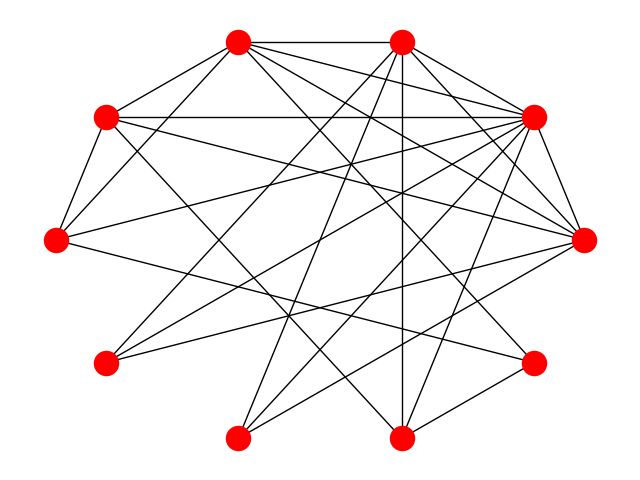
\includegraphics[width=.3\textwidth]{NonReplace.png}
	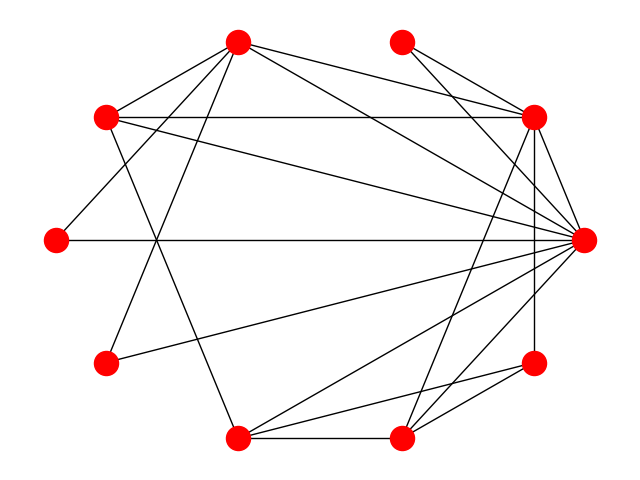
\includegraphics[width=.3\textwidth]{Replace.png}
	\caption{Left: \textit{Example graph of 10 nodes where we allows double edges(m=3). Not that there are nodes with degree less than m.}
		\\Right: \textit{Exampleof graph of 10 nodes. Note that all nodes have degree $>m$. Note that in both cases, I have not used $\mathcal{G}_0$, and instead have used a small initial graph to emphasise the difference in the cases.}}
\end{figure} 
This phenomena does not make sense in the circumstances for which this model is implemented, such as modeling the relationships between websites. Therefore I have decided to use the latter case. Also for large systems, theoretically there is no difference, since the probability of a node being chosen twice $\rightarrow 0$.
\subsection{Udpating Probabilities}
\\
\subsection{Testing}
\\
\section{Theoretical Derivation of Degree}
There are a few ways of approximated the degree distribution $p(k)$, all three of which use the master equation: 
\begin{equation}
n(k,t+1)=n(k,t)+m\Pi(k-1,t)n(k-1,t)-m\Pi(k,t)n(k,t)+\delta_{k,m}
\end{equation}
Where $\Pi(k,t)$ is the probaility of an edge being attached to a node of degree $k$.
Since we are taking $\Pi(k,t) \propto k$, and that the probabilities are normalised, way get that:
\begin{equation}
\Pi(k,t)=\frac{k}{\sum_{k=1}^{\infty}{kn(k,t)}}
\end{equation}
Where $kn(k,t)$ is the number of degrees of the nodes of degree k. Also, each edge is reponsible for 2 degrees, and so:
\begin{equation}
\Pi(k,t)=\frac{k}{2E(t)}}
\end{equation}
I have already discussed that $E(t)=mN(t)$ using the initial conditions chosen, and so $\Rightarrow \Pi(k,t)=\frac{k}{2mN(t)}$. Applying this to (1) the master equation becomes:
\begin{equation}
n(k,t+1)=n(k,t)+\frac{(k-1)n(k-1,t)}{2N(t)}-\frac{kn(k,t)}{2N(t)}+\delta_{k,m}
\end{equation}
Now we define the probability of choosing a degree randomly with degree $k$ at time $t$: 
\begin{equation}
p(k,t)=\frac{n(k,t)}{N(t)}\\
\end{equation}
So the master equation:
\begin{equation}
N(t+1)p(k,t+1)-N(t)p(k,t)=-\frac{k}{2}p(k-1,t)-\frac{k}{2}p(k,t)+ \delta_k,m
\end{equation}
\\NOT SURE HERE\\
In order to go further, we assume that $p(k)$ has nice ergodic properties. This means that $p_{\infty}=lim_{t \rightarrow \infty} p(k,t)$\\, i.e. the limit converges. Applying this to (6) the final form of our master equation becomes:
\begin{equation}
p_{\infty}(k)=-\frac{1}{2}((k-1)p_{\infty}(k-1)-kp_{\infty}(k)) +\delta_{k,m}
\end{equation}
\subsection{Continuous Approximation}
Equation (7) can be used to find the degree distribution of the model.
An approximation of this distribution can be found using a limiting case, e.i. instead of have descrete degrees, we look at the continuous case $k+1 \rightarrow k + \Delta k$. (7) becomes:
\begin{equation}
{p(k) \approx \lim\limits_{\Delta k \rightarrow 0}\frac{-\frac{1}{2}((k-\Delta k )p_{\infty}(k-\Delta k)-kp_{\infty}(k)) +\delta_{k,m}}{\Delta k} }
\end{equation}
\begin{equation}
\Rightarrow p(k)\approx \frac{\partial kp_{\infty}(k)}{\partial k}
\end{equation}
By inspection (Looking for a solution of the type $k^{-\gamma}$), we find that $p(k) \propto k^{-3}$ is a solution.  This solution is very approximal. However once case we would expect to see such a distribution is for $m \rightarrow \infty$. As $m$ grows large, the difference between $k-1$ and $k$ grows small proportional to $k$, and so the limiting case becomes a reality.
\subsection{Difference Derivation}
It is poosible however to derive a solution from the difference equation. First we look at $k>m$ and rearrange (7):
\begin{equation}
\frac{p_{\infty}(k)}{p_{\infty}(k-1)}=-\frac{k-1}{2(k+1)}
\end{equation}
This may no look particularly helpful, however there is an identity of the Gamma function. The equation:
\begin{equation}
\frac{f(z)}{f(z-1)}=\frac{z+a}{z+b}
\end{equation}
Has the solution
\begin{equation}
f(z)=A\frac{\Gamma(z+1+a)}{\Gamma(z+1+b)}
\end{equation}
Therefore our difference equation has solution
\begin{equation}
p_{\infty}(k)=A\frac{\Gamma(k)}{\Gamma(k+2)}
\end{equation}
Using the identity $\Gamma(n)=(n-1)!$ for $n \in \mathbb{N}_0
\section{Comparison with Real Data}
Now I wish to compare these theoretical plots with the actual data captured by my model.
I shall test the data for N=100,000 , so there is time for thr ergodic properties assumed to be completed. I shall run my programme for m=1,2,3. 
shows below is that 
-statisitical- chi squared, R^2, kolmogorov SMirnoff

\section{Largest K}
-How does it depend on N? Theoretical 4
-Real data
-Estimate uncertainties/errors

-data collapse?


\end{document}
